\chapter{Gerenciamento dos requisitos}

  \section{\textit{Backlogs}}
  
  Esta seção apresenta os \textit{Backlogs} dos níveis de Portfólio, Programa e Time, respectivamente. Nas Figuras é possível, também, visualizar os
  atributos de requisitos inerentes.
  
    \subsection{\textit{Backlog} Portfólio}
    
     A Figura \ref{fig:backlog_portifolio}, ilustra os épicos presentes no \textit{Backlog} do portfólio na ferramenta \textit{GatherSpace}.
      
       \begin{figure}[!htbp]
	\centering
	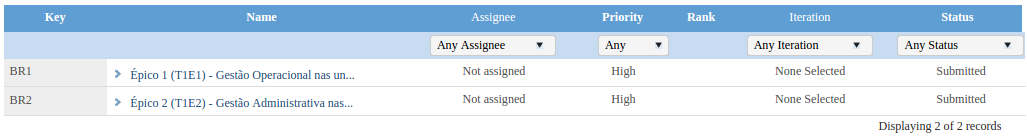
\includegraphics[scale=0.5, angle = 0]{figuras/backlog_portfolio}
	\caption[\textit{Backlog} Portfólio do Projeto]
	    {\textit{Backlog} Portfólio do Projeto.}
	\label{fig:backlog_portifolio}
      \end{figure}
    
    \subsection{\textit{Backlog} Programa}
    
   A Figura \ref{fig:backlog_programa}, ilustra as \textit{features} presentes no \textit{Backlog} do programa na ferramenta \textit{GatherSpace}.
    
       \begin{figure}[!htbp]
	\centering
	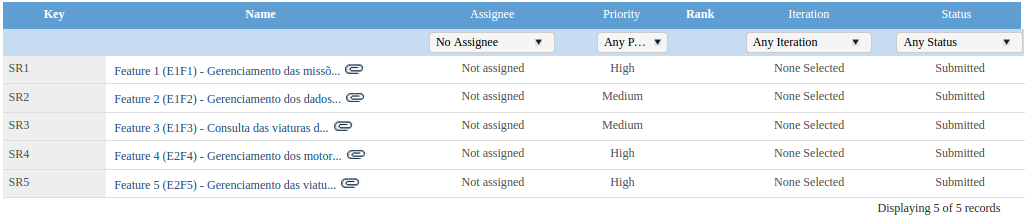
\includegraphics[scale=0.5, angle = 0]{figuras/backlog_programa}
	\caption[\textit{Backlog} Programa do Projeto]
	    {\textit{Backlog} Programa do Projeto.}
	\label{fig:backlog_programa}
      \end{figure}
    
    \subsection{\textit{Backlog} Time}
    
   As Figuras \ref{fig:backlog_time_1} e \ref{fig:backlog_time_2} , ilustram os casos de uso presentes nos \textit{Backlogs} do time na ferramenta \textit{GatherSpace}.
    
       \begin{figure}[!htbp]
	\centering
	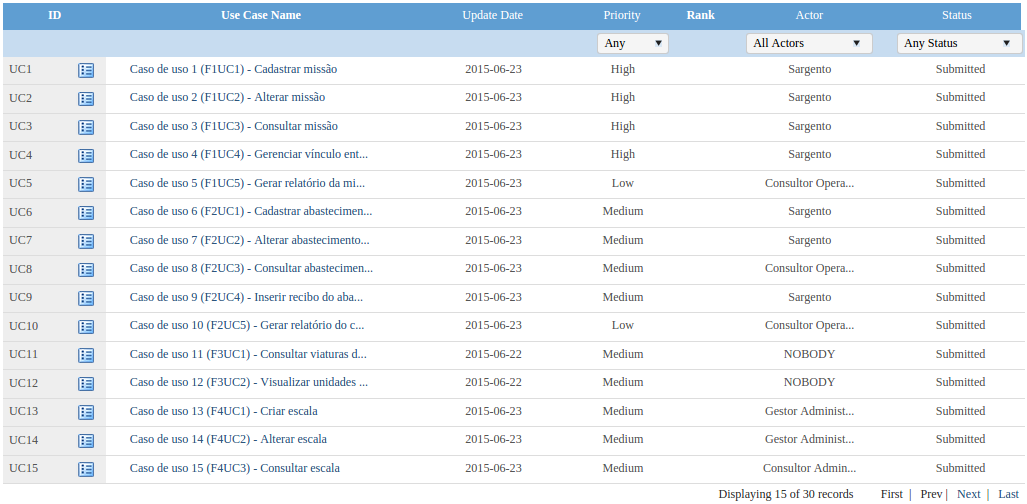
\includegraphics[scale=0.5, angle = 0]{figuras/backlog_time_1}
	\caption[\textit{Backlog} Time 1 do Projeto]
	    {\textit{Backlog} Time 1 do Projeto.}
	\label{fig:backlog_time_1}
      \end{figure}
      
       \begin{figure}[!htbp]
	\centering
	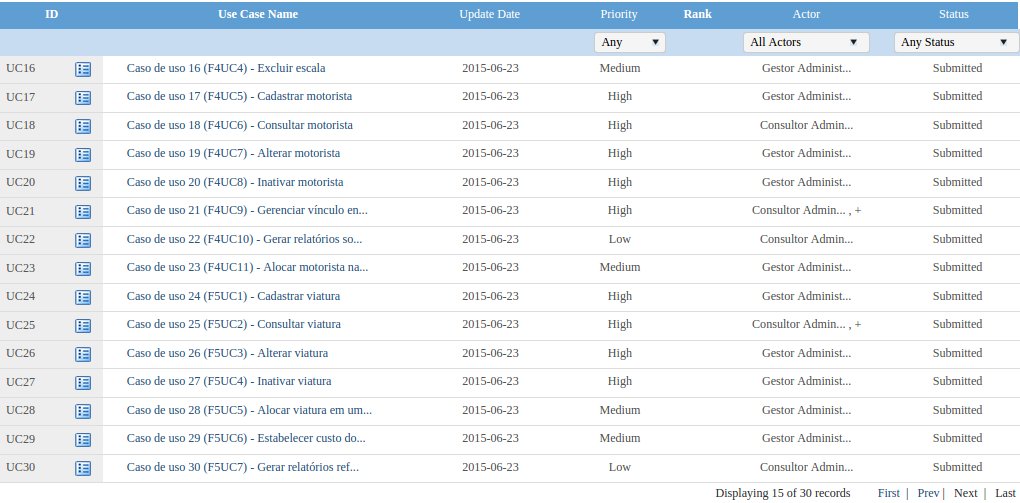
\includegraphics[scale=0.5, angle = 0]{figuras/backlog_time_2}
	\caption[\textit{Backlog} Time 2 do Projeto]
	    {\textit{Backlog} Time 2 do Projeto.}
	\label{fig:backlog_time_2}
      \end{figure}
     
  
  \section{Matriz de rastreabilidade}
  
    A Figura \ref{fig:matriz_rastreabilidade} ilustra a matriz de rastreabilidade dos requisitos do projeto gerada pela ferramenta
   \textit{GatherSpace}. Nela é possível ter uma visão ampla da rastreabilidade entre todos os requisitos do sistema.  
  
      \begin{figure}[!htbp]
	\centering
	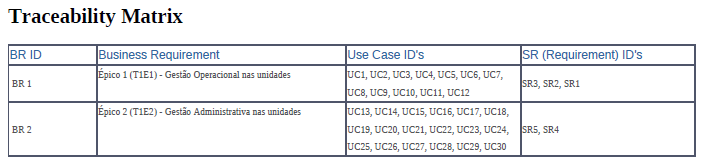
\includegraphics[scale= 0.9, angle = 0]{figuras/matriz_rastreabilidade}
	\caption[Matriz de rastreabilidade dos requisitos [\textit{GatherSpace]}]
	    {Matriz de rastreabilidade dos requisitos [\textit{GatherSpace]}.}
	\label{fig:matriz_rastreabilidade}
      \end{figure}
  
  \section{Árvore de rastreabilidade}
  
  Esta seção apresenta a árvore de rastreabilidade de requisitos do projeto (Figura \ref{fig:arvore_rastreabilidade}) onde é ilustrada
  a rastreabilidade vertical dos requisitos. A partir do tema, são derivados os épicos, que por sua vez derivam as \textit{features}
  e por fim, destas são derivados os casos de uso.
  
    \begin{figure}[!htbp]
	\centering
	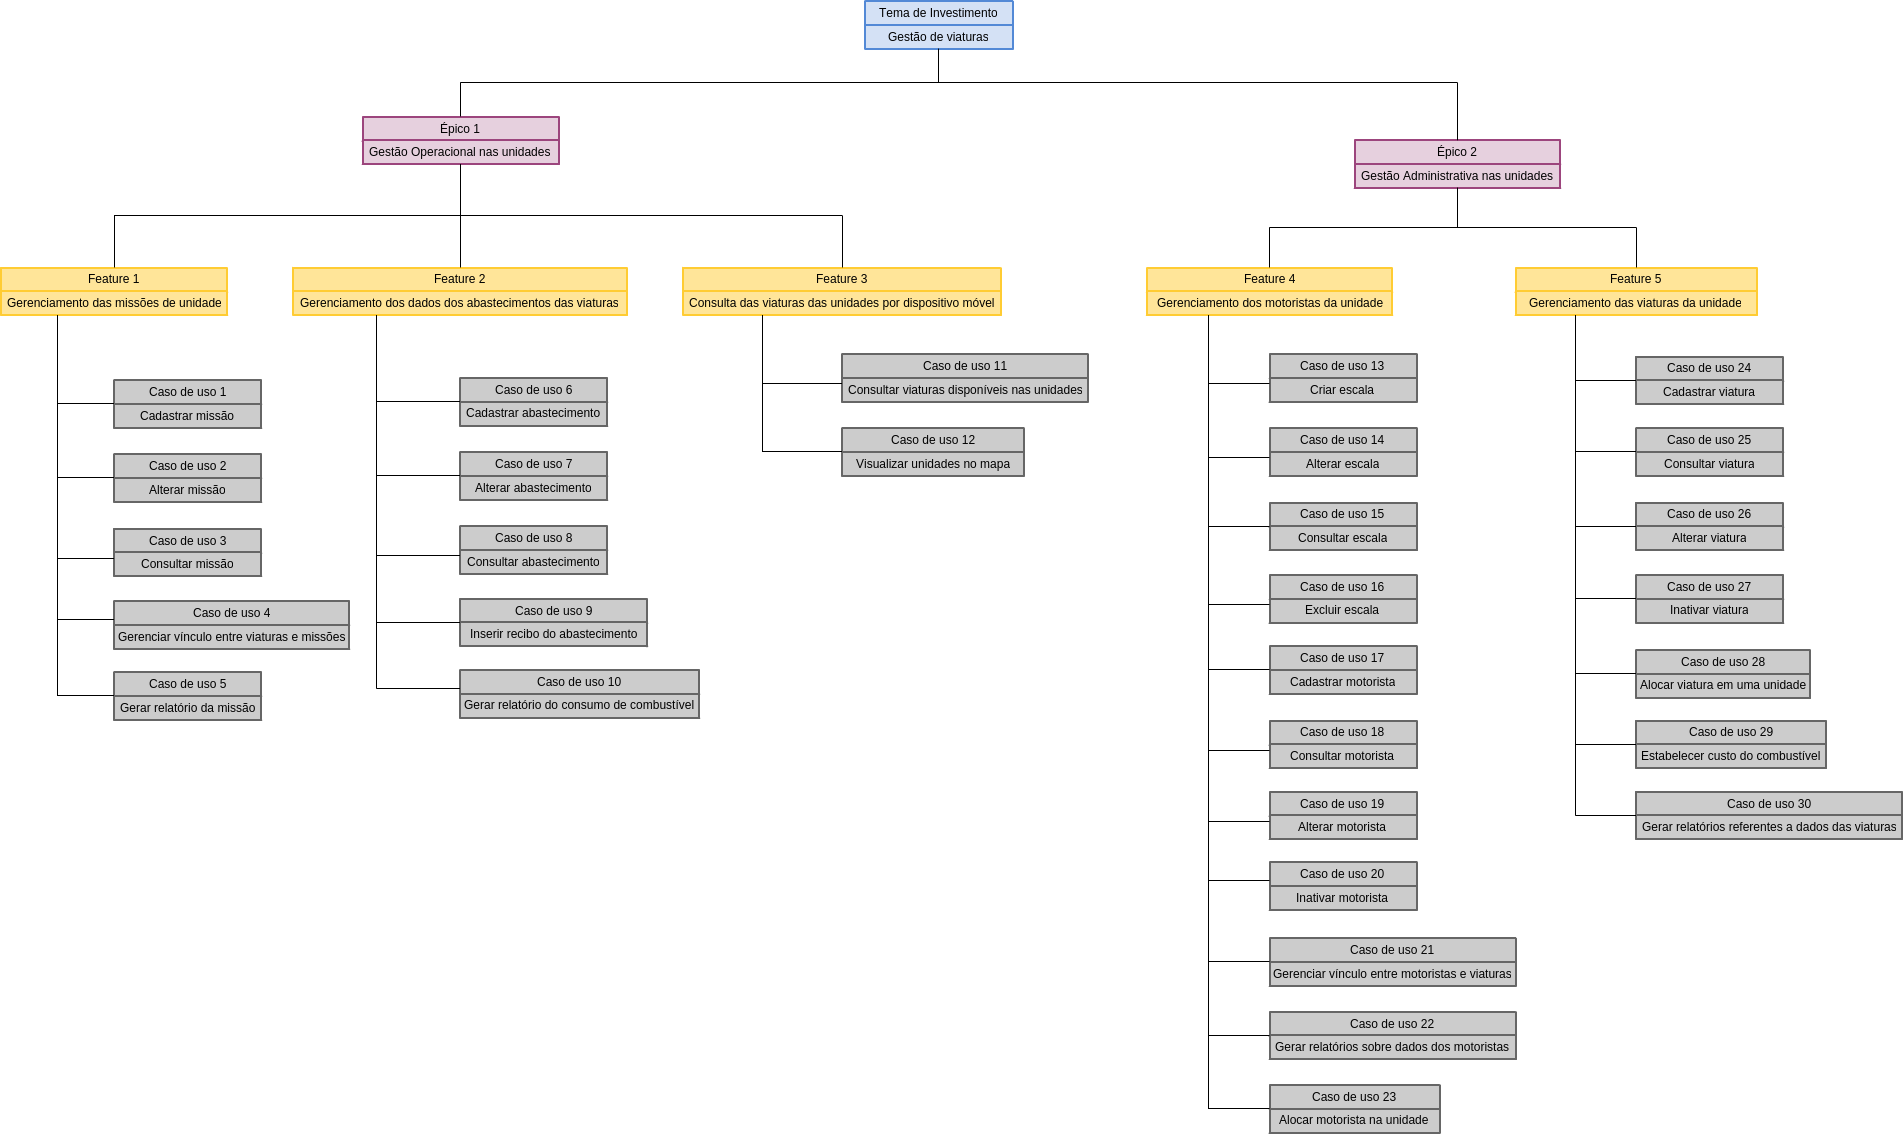
\includegraphics[scale=0.35, angle = 90]{figuras/arvore_rastreabilidade}
	\caption[Árvore de rastreabilidade dos requisitos do projeto]
	    {Árvore de rastreabilidade dos requisitos do projeto}
	\label{fig:arvore_rastreabilidade}
      \end{figure}